\cleardoublepage%
\chapter{\label{chap:intro}Theory}%


\section{\label{sec:intro_swm_africa}Optical Fibre}%
Optical fiber, a remarkable technology in modern telecommunications and data transmission, is a slender, flexible, and transparent strand made of ultra-pure glass or plastic. At its core, optical fiber operates on the principles of physics, primarily utilizing total internal reflection. When light, typically in the form of laser or LED-generated pulses, enters the fiber at a certain angle within the core, it is continually reflected off the inner walls due to the higher refractive index of the core compared to the surrounding cladding. This mechanism traps the light within the core, allowing it to travel great distances with minimal signal loss. The physics behind optical fibers enable them to transmit data at nearly the speed of light, making them an essential component in the modern world of high-speed internet, telecommunications, and data networking.

\section{\label{sec:intro_res_quest}Experiments}


\subsection{\label{sec:intro_level3}Bending Loss Experiment}
In a bending loss experiment on optical fiber, the objective is to understand how the curvature of the fiber affects the transmission of light signals. Optical fibers are designed to efficiently transmit light in straight paths, but when they are bent, some of the light can escape due to bending-induced micro bending or macro bending. This experiment typically involves subjecting the optical fiber to various bending radii and angles while measuring the attenuation of the transmitted light. By quantifying the bending losses, researchers gain insights into the fiber's resilience to bending and the minimum bend radius that can be tolerated before signal quality significantly deteriorates. This knowledge is crucial for optimizing fiber optic network layouts and ensuring reliable data transmission, especially in scenarios where bending of optical fibers cannot be avoided.\\
Here, in this experiment we took a bending loss apparatus consisting of rings of different diameters(35 mm, 45 mm, 55 mm, 65 mm) and took turn(s) of the optical fibre to measure the attenuation of laser passing through it and which was detected at the photo diode detector end.\\
\begin{figure}
    \centering
    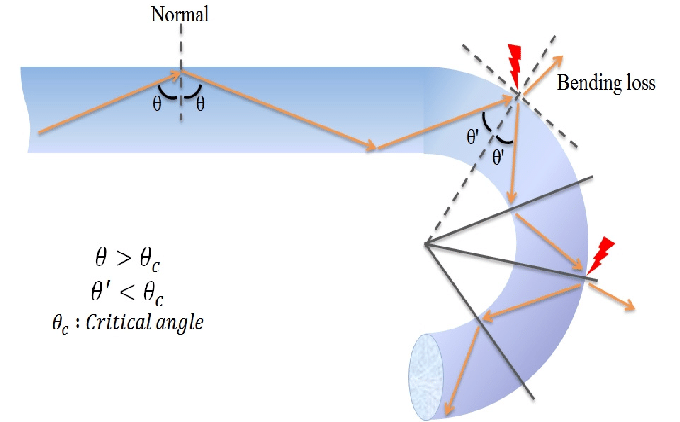
\includegraphics[scale=0.5]{chapters/Schematic-diagram-of-the-bending-loss-in-a-bent-optical-fiber.png}
    \caption{Bending Loss in a Optical Fiber}
\end{figure}
\subsection{\label{sec:intro_level3}Calculation of Numerical Aperature}
 A single-mode optical fiber will only propagate light that enters the fiber within a certain Cone, known as the acceptance cone of the fiber. The half-angle of this cone is called the acceptance angle ($\theta_{a}$) \\
    So, the Acceptance angle is defined by \\
    $$ \theta_{a} = \tan^{-1}\frac{D}{Z}$$
    and the Numerical Aperture is defined by,
    $$ NA = \sin{\theta_{a}} $$ \\
\begin{figure}
    \centering
    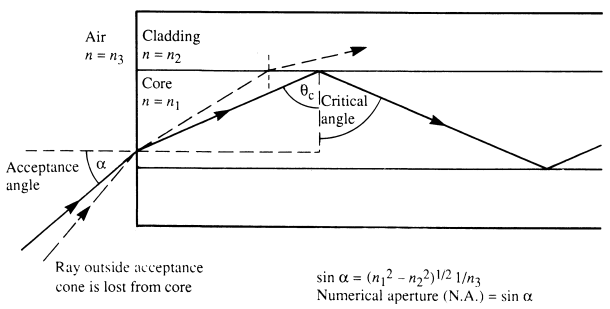
\includegraphics[scale=1]{chapters/image4.png}
    \caption{Numerical Aperature Calculation of Optical Fiber}
\end{figure}
The numerical aperture (NA) of an optical fiber is a key parameter that characterizes its ability to gather and transmit light. It is calculated using the formula NA = n * $\sin(\theta)$, where "n" is the refractive index of the core of the fiber, and $"\theta"$ is the half-angle of the maximum cone of light that can enter or exit the fiber while undergoing total internal reflection. The numerical aperture provides critical information about the fiber's light-capturing and light-gathering capabilities. A higher NA indicates a fiber's ability to collect light from a wider range of angles, making it more suitable for applications where efficient light transmission and coupling are essential, such as in high-speed data communication or medical imaging systems. Calculating the numerical aperture is fundamental in designing and selecting optical fibers tailored to specific optical systems and applications.
\subsection{\label{sec:intro_level3}Splicing Loss Experiment}
In a splice loss experiment on optical fiber, the objective is to quantify the attenuation or signal loss that occurs when two optical fibers are joined or spliced together. This experiment typically involves aligning the ends of two fiber segments with high precision and using specialized fusion splicing equipment. The key mathematical calculations involve measuring the power of the transmitted light before and after the splice. By comparing these power levels, researchers can determine the splice loss, expressed in decibels (dB), which represents the reduction in signal strength due to the splice. 
\begin{figure}
    \centering
    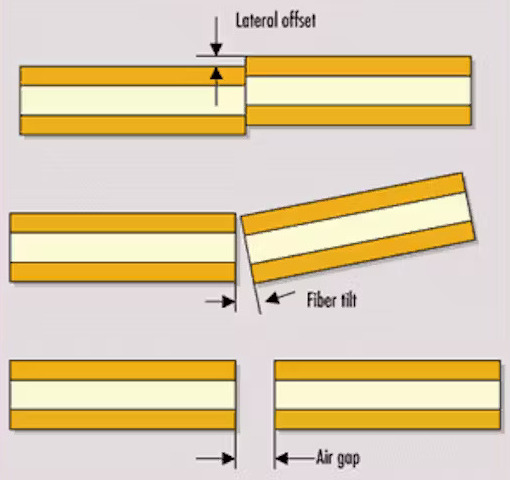
\includegraphics[scale=0.7]{chapters/splice.jpg}
    \caption{Splice Loss in Optical Fiber}
\end{figure}
Understanding splice losses is crucial for optimizing the efficiency and reliability of fiber optic networks, as it helps in selecting appropriate splicing techniques and minimizing signal degradation during the connection of optical fibers.